\begin{tikzpicture}
  \node[anchor=south west,inner sep=0](image) at (0,0) {
    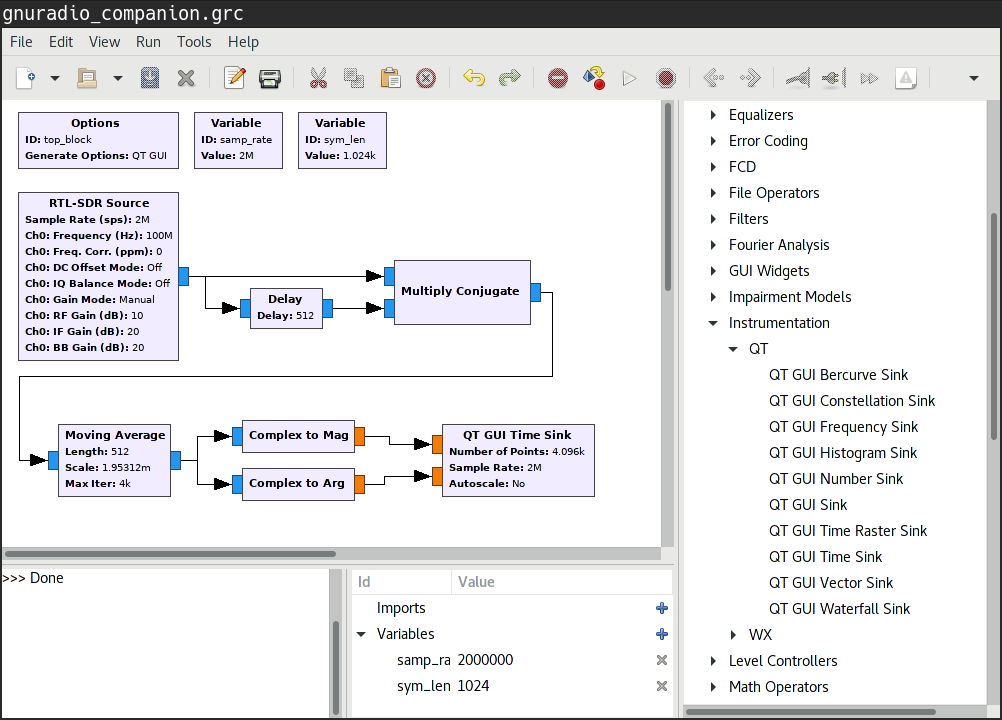
\includegraphics[width=\linewidth]{images/gnuradio_companion.png}
  };

  \begin{scope}[x={(image.south east)},y={(image.north west)}]
    \draw[red, thick, rounded corners] (0.0175, 0.8451) rectangle (0.1791, 0.7646); % Options
    \draw[red, thick, rounded corners] (0.1931, 0.8451) rectangle (0.3867, 0.7646); % Named Variables
    \draw[red, thick, rounded corners] (0.0175, 0.7340) rectangle (0.5943, 0.3035); % Flowgraph
    \draw[red, thick, rounded corners] (0.6831, 0.8590) rectangle (0.9835, 0.0229); % Available blocks

    \draw[red, thick]
    (0.0175, 0.80485) -- (-0.07, 0.80485) node[anchor=east, black, align=right]{Flowgraph\\options}
    (0.0175, 0.51875) -- (-0.07, 0.51875) node[anchor=east, black, align=right]{Flowgraph}
    (0.9835, 0.44095) -- ( 1.07, 0.44095) node[anchor=west, black, align=left]{Available\\blocks}
    (0.2899, 0.84510) -- (0.2899, 0.92) -- (-0.07, 0.92) node[anchor=east, black, align=right]{Named\\Variables};
  \end{scope}
\end{tikzpicture}
